\appendix
\section{Magnitude Distributions}\label{sec:selection}
Figure~\ref{fig:selection} compares the photometric training population
with the spectroscopic training and test samples. Spectroscopy favors
brighter galaxies even though the photometric selection does not require
a spectroscopic redshift. The test metrics therefore describe the
spectroscopic subset of our magnitude-limited population.

\begin{figure}[ht]
\centering
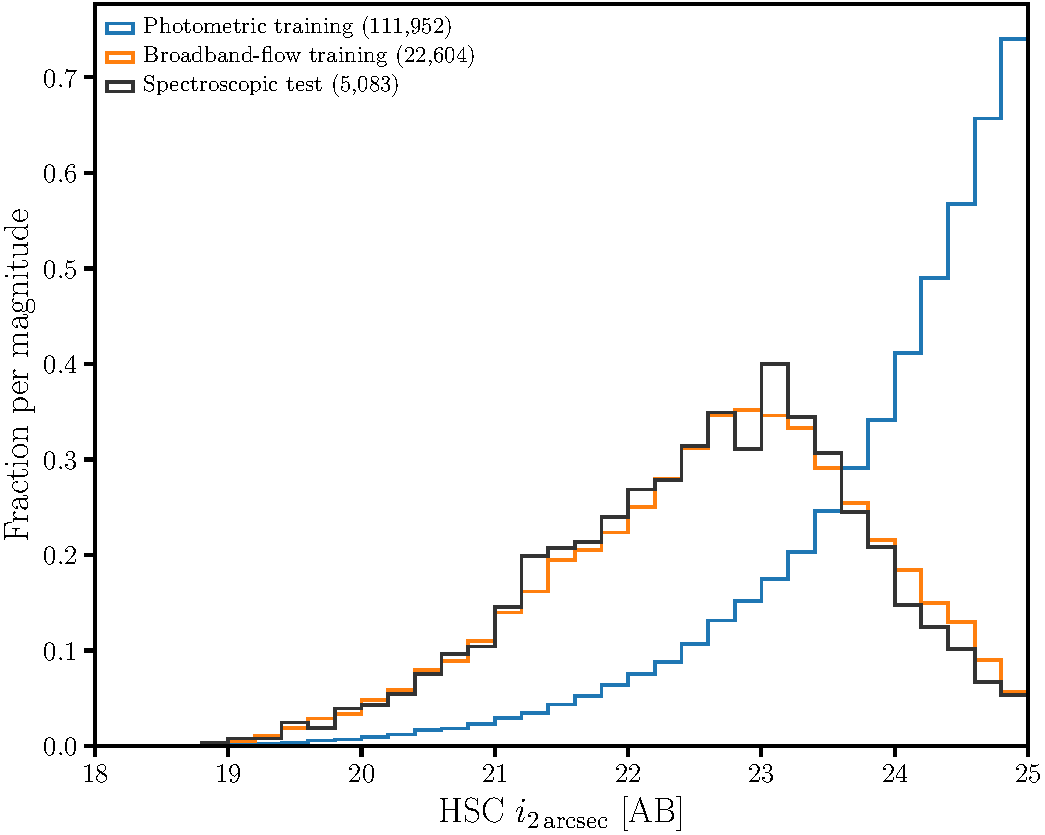
\includegraphics[width=0.55\textwidth]{figures/fig01_selection.pdf}
\caption{\label{fig:selection}
Native HSC $i$-band aperture magnitudes for the full photometric training
sample, broadband-flow spectroscopic training sample, and spectroscopic
test sample. Histograms are normalized separately. The displayed
$18<i<25$ range imposes no additional bright cut.}
\end{figure}
